% ============= CHAPTER 6: USER MANUAL =============
\chapter{User Manual}
\label{ch:chapter6}

\section{Chapter Overview}

Chapter 6 documents the operational user interface of the TIBSA (Threat Intelligence and Breach Security Analysis) platform. TIBSA integrates vulnerability assessment, infrastructure threat intelligence, malware analysis, and architectural threat modelling within a unified analyst workspace accessible through the TIBSA Shield console. The following sections describe authentication, navigation, core analytical modules, reporting, administration, and cross-module reference material. This manual focuses on user actions, expected outputs, and operational workflows rather than backend implementation details.

\section{System Access and Authentication}

TIBSA employs Supabase Auth with a FastAPI backend for credential validation, profile provisioning, and role enforcement. All analytical modules require an authenticated session.

\subsection{Public Landing Page}

Unauthenticated users access the platform at the root URL, which presents branding, capability summary, and navigation to login and registration. No analytical functionality is exposed prior to authentication.

Login and Get Started controls route to /login and /register respectively. Authenticated users visiting the root URL are redirected to the dashboard.

\begin{figure}[H]
\centering
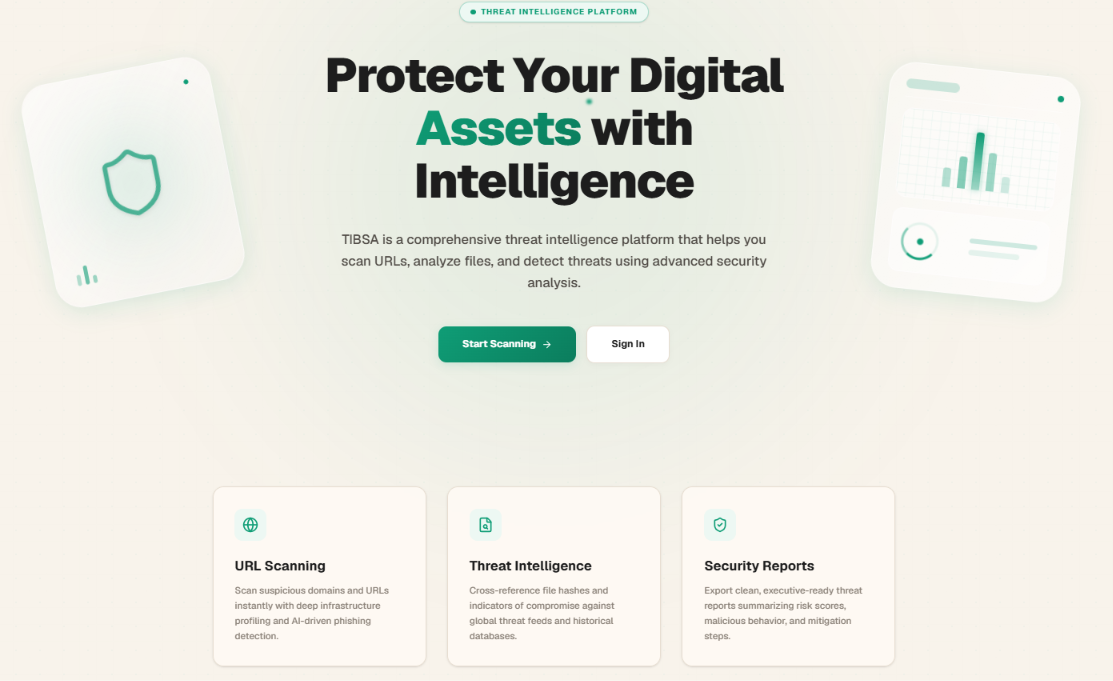
\includegraphics[width=\textwidth]{media/TIBSA Public Landing Page.png}
\caption{TIBSA Public Landing Page}
\label{fig:ch6_tibsa_public_landing_page}
\end{figure}

\subsection{Registration and Login}

Registration requires full name, valid email, and a password meeting the twelve-character complexity policy (uppercase, lowercase, numeric, and special characters). Login accepts email and password via POST /api/v1/auth/login, returning a JWT bearer token. Google and GitHub OAuth are supported through Supabase. Registration is rate-limited to three requests per minute; login to five per minute. Failed authentication returns generic error messages to prevent user enumeration.

OAuth users receive automatically provisioned profiles on first authentication. Token refresh is supported via POST /api/v1/auth/refresh for session continuity.

\begin{figure}[H]
\centering
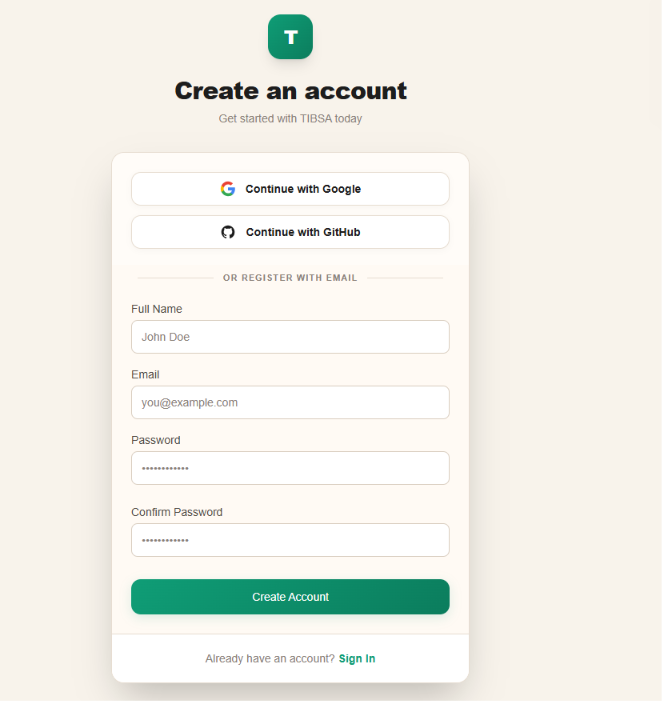
\includegraphics[width=\textwidth]{media/Registration and Login Interface.png}
\caption{Registration and Login Interface}
\label{fig:ch6_registration_and_login_interface}
\end{figure}

\subsection{Session Management}

Upon authentication, the platform retrieves the user profile from GET /api/v1/users/me. Session state is maintained through Supabase AuthContext listeners. Users sign out via the header profile menu, invoking POST /api/v1/auth/logout. Deactivated accounts (is\_active = false) are redirected to the suspended-account page and cannot access protected routes.

Protected routes employ RoleGuard verification before rendering module content. Expired tokens require full reauthentication through the login interface.

\subsection{Roles and Permissions}

Two roles are implemented: user and admin. Standard users access dashboard analytical modules. Administrators additionally access the SOC Nexus console at /admin for user management, threat feeds, analytics, system health, audit logs, and platform settings. Role enforcement is applied through RoleGuard components on protected routes.

Role changes are performed by administrators through the User Management interface in SOC Nexus. Standard users cannot access /admin routes.

\section{Platform Navigation and Global Interface}

Authenticated users operate within a persistent layout comprising sidebar, header, content area, footer, and floating AI assistant.

\subsection{Sidebar Navigation}

The collapsible sidebar provides links to Dashboard, Investigations, Infra Intelligence, Scans, Penetration Testing, Threats, Threat Modeling, AI Analysis, Reports History, and Profile. Collapse state persists in browser localStorage. The active route is highlighted for orientation.

The Threats link opens on-demand Threat Intelligence Lookup for rapid IOC reputation verification without full Infra Intelligence pipeline execution.

\subsection{Header and Notifications}

The header displays platform branding, breadcrumb navigation, a notification bell, and profile controls. Notifications are fetched from GET /api/v1/notifications/ with fifteen-second auto-refresh. Users may mark individual or all notifications as read.

The profile dropdown provides access to Profile and Sign Out controls. Breadcrumb trails are constructed dynamically from the active route pathname.

\subsection{AI Assistant and Admin Switcher}

A floating AI Security Assistant chatbot provides contextual security guidance across dashboard routes. Administrators access a console switcher to toggle between TIBSA Shield (analyst) and SOC Nexus (administration) interfaces.

The AI assistant accepts natural-language security queries and is available on all dashboard routes via the floating action button.

\begin{figure}[H]
\centering
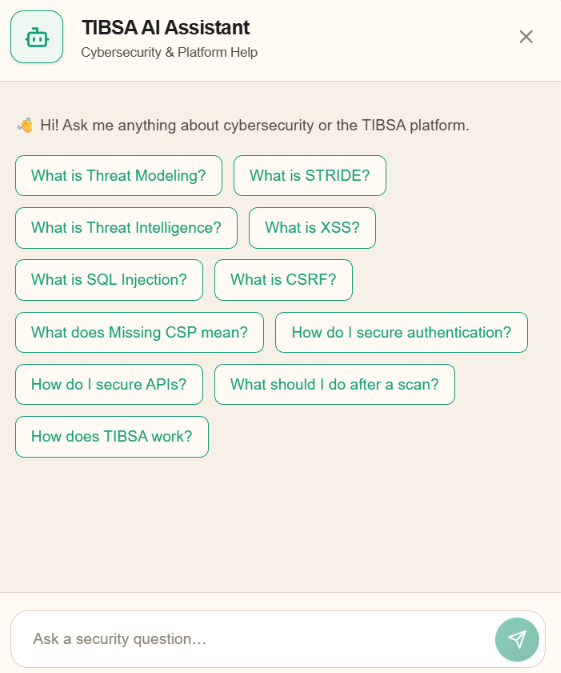
\includegraphics[width=\textwidth]{media/AI Assistant and Admin Console Switcher.png}
\caption{AI Assistant and Admin Console Switcher}
\label{fig:ch6_ai_assistant_and_admin_console_switcher}
\end{figure}

\section{Main Dashboard}

The main dashboard at /dashboard serves as a workflow-oriented module launcher rather than a metrics dashboard.

\subsection{Dashboard Overview}

The dashboard displays a personalised welcome banner and platform summary. It provides direct entry to investigation pipelines and standalone services without intermediate configuration.

Account status is verified via GET /api/v1/users/dashboard/stats on page load. Deactivated accounts are redirected before module content renders.

\begin{figure}[H]
\centering
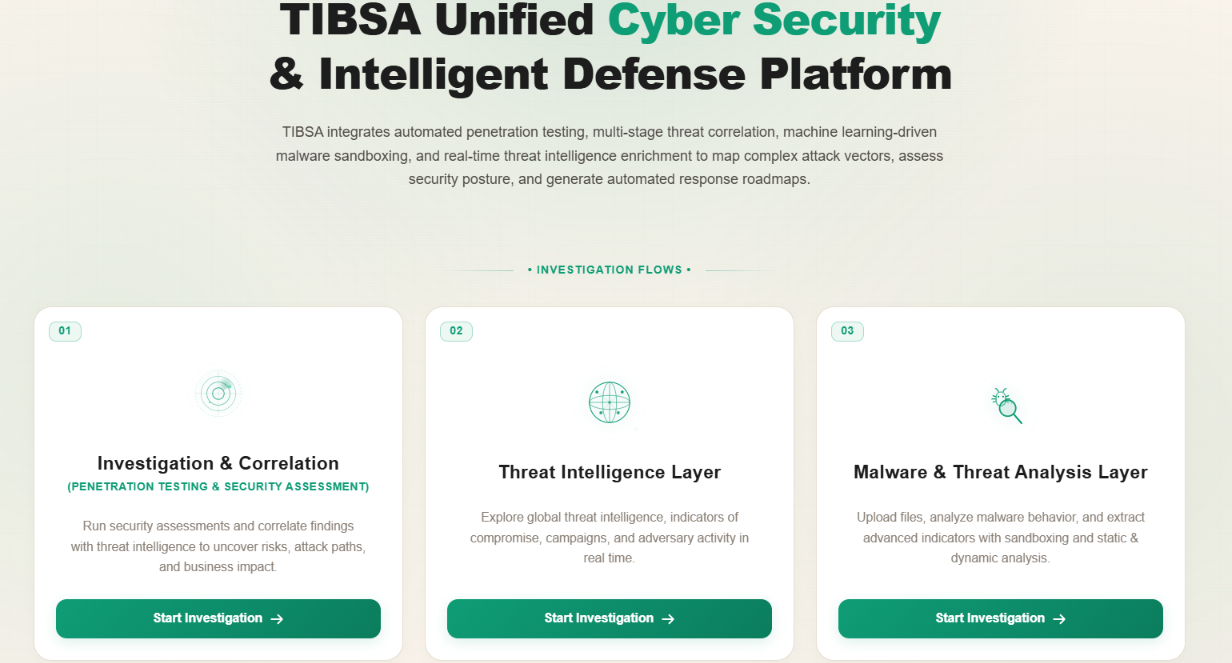
\includegraphics[width=\textwidth]{media/main dashboard.png}
\caption{Main Dashboard}
\label{fig:ch6_main_dashboard}
\end{figure}

\subsection{Investigation Flow Cards}

Three flow cards launch Security Investigations (URL-targeted pipeline), Infra Intelligence (IOC enrichment), and AI Malware Analysis (file upload). Each card provides a Start Investigation button routing to the respective module.

Each card uses distinct colour theming (blue, emerald, purple) to differentiate investigation paradigms at a glance.

\subsection{Standalone Security Services}

Six shortcut tiles provide rapid access to Scans, Penetration Testing, Threat Intelligence Lookup, Threat Modeling, Reports History, and Profile without entering a full investigation pipeline.

Tiles route directly to module entry points, bypassing the multi-stage pipeline orchestration used by investigation flow cards.

\subsection{Dashboard UX and Design Logic}

The workflow-driven design prioritises module discovery over aggregate telemetry display. Analytical depth resides within individual module workspaces.

This design supports SOC workflows where analysts select the appropriate tool based on indicator type rather than monitoring aggregate platform metrics.

\section{Security Investigations}

Security Investigations execute a multi-stage URL-targeted pipeline combining penetration testing, threat intelligence, correlation, and AI reporting at /dashboard/investigations. This module represents the platform's primary integrated assessment workflow, orchestrating multiple analytical stages within a single investigation context linked to a submitted URL.

\subsection{Launching a Security Investigation}

Submit a target URL on the investigations page. The platform validates the URL format and creates an investigation record. Only URL targets are supported.

The investigations list page displays prior runs with filtering by status and chronological ordering for quick access to active or completed pipelines.

\subsection{Investigation Execution and Live Monitoring}

The pipeline executes stages sequentially: penetration testing, threat lookup, correlation, and AI summary generation. Progress is displayed in real time on the investigation detail page. Users may stop an active investigation.

Stage completion timestamps and status badges enable analysts to identify bottlenecks or failed stages requiring intervention.

\begin{figure}[H]
\centering
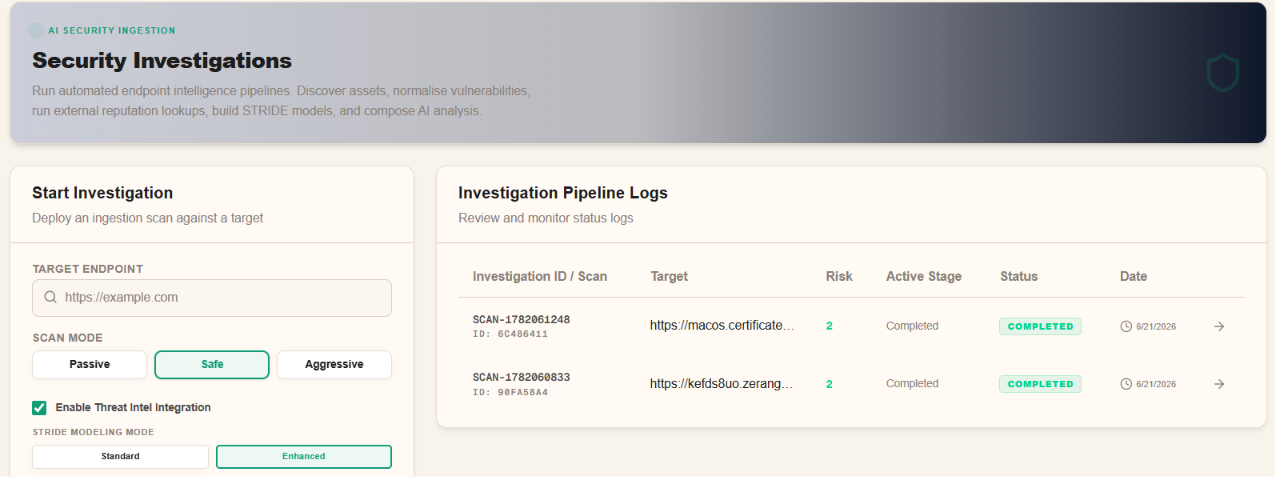
\includegraphics[width=\textwidth]{media/Security Investigation Pipeline.png}
\caption{Security Investigation Pipeline}
\label{fig:ch6_security_investigation_pipeline}
\end{figure}

\subsection{Results and Analysis Tabs}

Completed investigations present tabbed results including scan findings, threat intelligence enrichment, correlation analysis, and AI-generated executive summary.

Each tab presents deterministic scan output alongside correlated threat intelligence data where available from integrated feeds.

\subsection{Investigation Report Export}

Export completed investigations as JSON (structured data) or PDF (executive report) from the investigation detail workspace.

JSON exports support downstream SIEM integration; PDF exports provide formatted executive summaries suitable for stakeholder reporting.

\subsection{Investigation History and Management}

The investigations list displays prior runs with status, risk score, and target. Select any entry to reopen the detail workspace or access Reports History.

Failed investigations retain partial results where stages completed before termination, supporting forensic review of incomplete assessments.

\section{Infra Intelligence}

Infra Intelligence performs eight-stage infrastructure IOC enrichment for domain, IP, URL, hash, and email targets at /dashboard/infra-investigations. The pipeline aggregates DNS, WHOIS, reputation, certificate, and heuristic data to produce a composite infrastructure risk assessment suitable for threat hunting and incident triage.

\subsection{Infra Intelligence Module Overview}

The module accepts heterogeneous indicators and executes DNS, WHOIS, reputation, certificate, and heuristic analysis stages to produce a composite risk assessment.

The Threat Intelligence Lookup module (/dashboard/threats) provides rapid on-demand reputation checks using the same IOC types without full pipeline execution.

\subsection{Launching an Infra Investigation}

Enter a target indicator on the launch page. Validation rejects empty inputs, targets exceeding 2048 characters, and private/loopback addresses.

The intake stage automatically classifies the indicator type (url, domain, ip, hash, email) and normalises the target for downstream enrichment queries.

\subsection{Infra Investigation Pipeline Execution}

Eight pipeline stages execute sequentially with live status updates. Each stage contributes enrichment data displayed on the investigation detail page.

Failed stages display error context on the detail page without preventing review of successfully completed enrichment stages.

\begin{figure}[H]
\centering
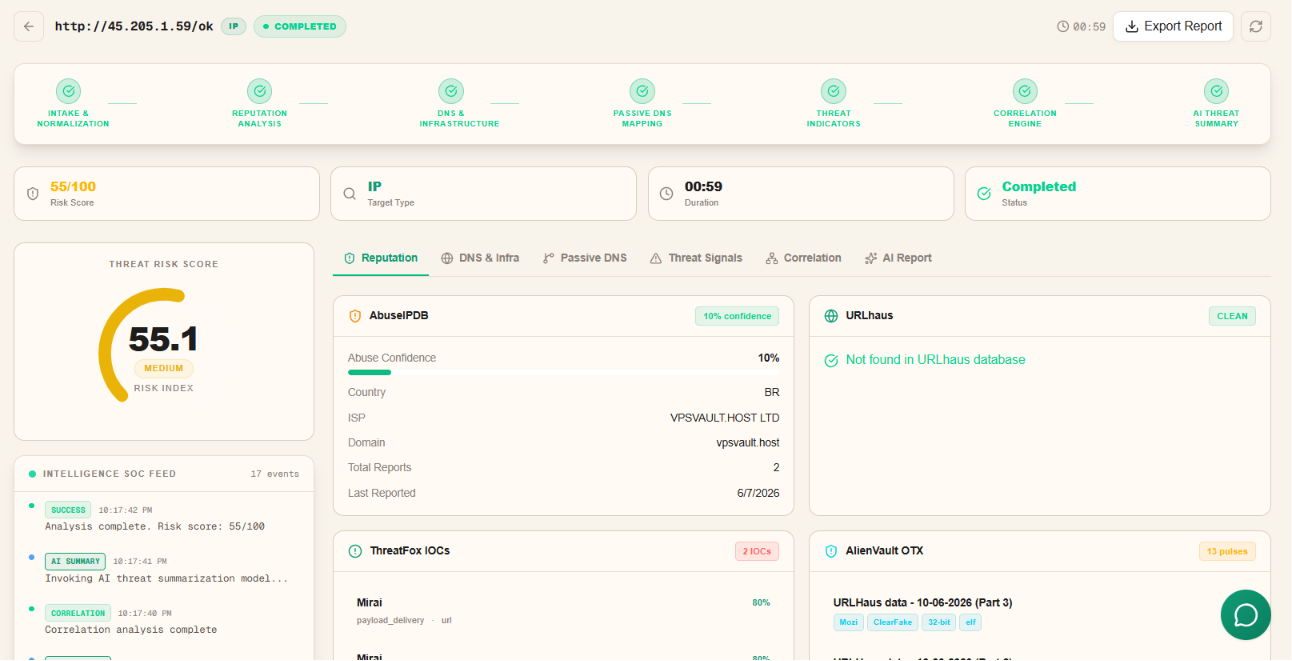
\includegraphics[width=\textwidth]{media/Infra Intelligence Pipeline.png}
\caption{Infra Intelligence Pipeline}
\label{fig:ch6_infra_intelligence_pipeline}
\end{figure}

\subsection{Results and Analysis Tabs}

Results are organised in tabbed panels covering intake, DNS, WHOIS, reputation, certificates, indicators, and AI-generated infrastructure report.

The AI report tab synthesises stage outputs into a narrative infrastructure assessment when generation completes successfully.

\subsection{Risk Scoring and Verdict Generation}

A composite risk score and verdict (e.g., benign, suspicious, malicious) are calculated from weighted stage outputs and displayed prominently on the detail page.

Risk thresholds are influenced by module settings stored in localStorage, including feed weights and keyword lists configured on the settings page.

\subsection{Infra Investigation History and Reports}

History and reports pages list completed investigations. Export PDF or JSON from the detail workspace. Module settings persist locally in browser localStorage.

The reports page provides a dedicated view for browsing completed investigations and accessing archived PDF outputs.

\section{Security Scans}

Security Scans provides VirusTotal-integrated URL and file reputation scanning at /dashboard/scans. The module supports asynchronous background scanning with automatic status polling, enabling analysts to submit multiple indicators concurrently.

\subsection{Security Scans Module Overview}

The module supports URL scanning, file upload scanning (max 32 MB), and hash-only lookup (MD5, SHA-1, SHA-256). Scans execute in the background with status polling.

Scan submission returns immediately; results populate asynchronously as VirusTotal processing completes. The interface auto-refreshes every five seconds while scans are active.

\begin{figure}[H]
\centering
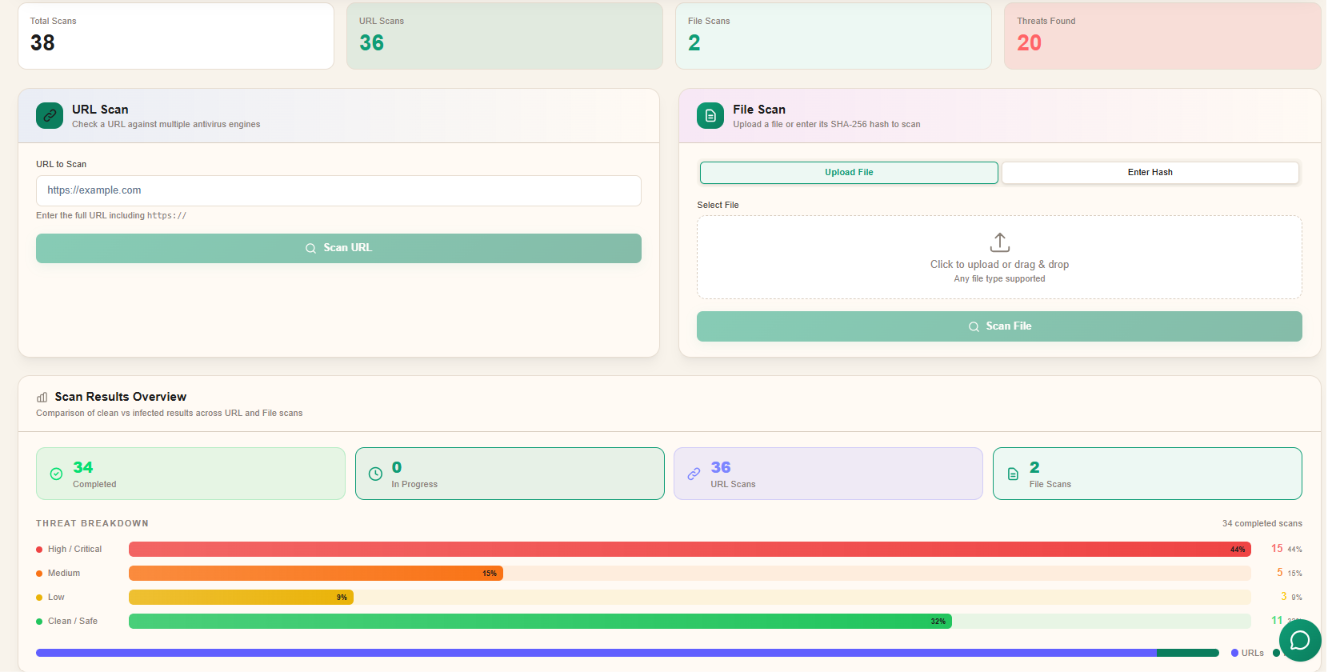
\includegraphics[width=\textwidth]{media/Security Scans Interface.png}
\caption{Security Scans Interface}
\label{fig:ch6_security_scans_interface}
\end{figure}

\subsection{URL Scanning}

Submit URLs beginning with http:// or https://. Results display engine detection counts and threat classification upon completion.

Client-side validation requires URLs to include an explicit http:// or https:// scheme before submission is permitted.

\subsection{File Scanning and Hash Analysis}

Upload files directly or submit a known hash for reputation lookup without file transfer. File uploads are limited to 32 MB.

Hash mode accepts MD5, SHA-1, or SHA-256 values, computing hashes client-side when a file is selected in upload mode for reference.

\subsection{Scan Results Interpretation}

Results present detection ratios, engine verdicts, and threat level classification (benign, suspicious, malicious). Detailed engine breakdowns are available in the scan detail modal.

Detection ratios below vendor consensus thresholds may still warrant manual review when contextual risk factors apply.

\subsection{Scan History and Management}

Scan history supports filtering by URL and file scans. Active scans may be cancelled; completed scans can be reviewed or deleted.

Cancelled scans display a distinct status badge. Delete controls remove entries from the user scan history.

\section{Penetration Testing}

Penetration Testing provides standalone website vulnerability scanning at /dashboard/website-scanner, accepting URL targets only. The scanner executes automated security tests and categorises findings by severity for prioritised remediation.

\subsection{Penetration Testing Module Overview}

The module executes automated security tests including header analysis, cookie review, SSL/TLS assessment, and vulnerability detection against submitted URLs.

Unlike Security Investigations, this module executes website scanning independently without threat correlation or AI summary stages.

\subsection{Configuring a Penetration Test}

Enter the target URL and submit. Configuration is minimal; the scanner applies default test modules automatically.

Only publicly accessible URLs should be submitted; internal addresses are outside the module's intended scope.

\subsection{Executing the Website Scan}

The scan runs asynchronously with progress indication. Findings are categorised by severity (critical, high, medium, low, informational).

Scan duration varies with target complexity and response latency. Progress indicators update as individual test modules complete.

\begin{figure}[H]
\centering
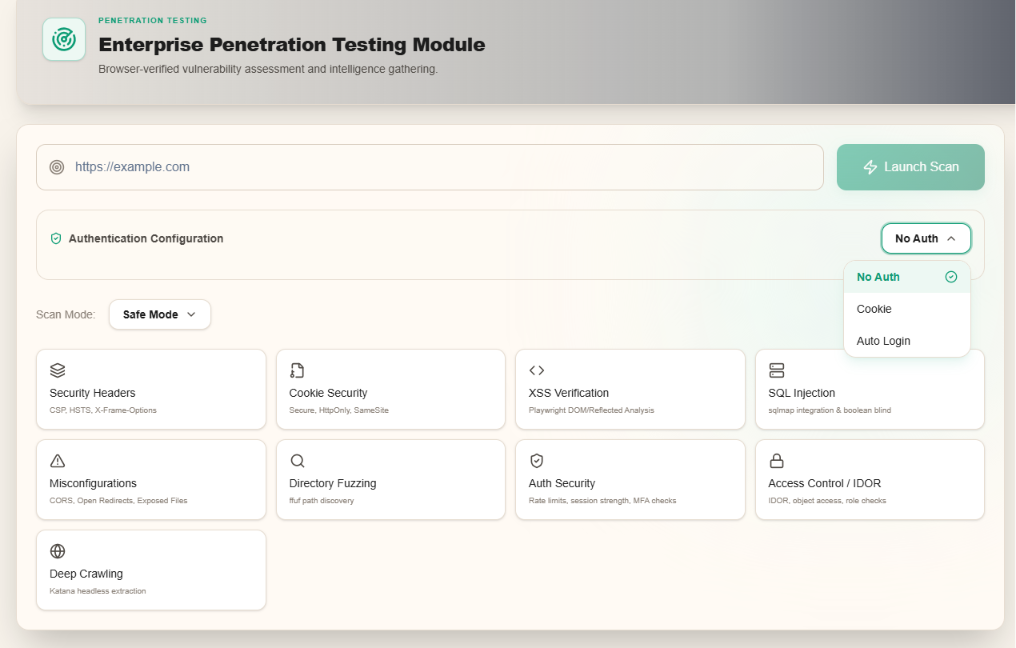
\includegraphics[width=\textwidth]{media/Penetration Testing Results.png}
\caption{Penetration Testing Results}
\label{fig:ch6_penetration_testing_results}
\end{figure}

\subsection{Reviewing Penetration Testing Results}

Results display findings with descriptions, evidence, and remediation recommendations. A summary risk score reflects overall posture.

Findings are expandable to reveal technical evidence including header values, cookie attributes, and certificate details.

\subsection{Exporting and Reviewing Scan Results}

Export scan data as JSON for integration or review in the dedicated review page. JSON is cached in localStorage for client-side review.

The review page at /dashboard/website-scanner/review loads cached JSON from localStorage for offline-capable result inspection.

\subsection{Penetration Testing History}

Prior scans are listed with target, status, and date. Access via module history or Reports History.

Completed scans appear in Reports History under the Penetration Testing tab with target URL, status, and completion date.

\section{Threat Modeling}

Threat Modeling applies STRIDE methodology to application design profiles at /dashboard/threat-modeling without requiring live target scanning. The module supports proactive security assessment during application design and architecture review phases.

\subsection{Threat Modeling Module Overview}

Users configure an application profile (technology stack, authentication method, data sensitivity) and generate STRIDE-based threat analysis.

Threat Modeling operates independently of live target scanning, evaluating application design characteristics through declarative profile configuration.

\subsection{Application Profile Configuration}

Complete the profile form specifying application name, architecture type, framework, authentication, and deployment model. Preset templates accelerate configuration.

Profile fields include application name, description, architecture pattern, programming language, framework, authentication mechanism, and data classification.

\subsection{Threat Analysis Generation}

Submit the profile to generate threats across Spoofing, Tampering, Repudiation, Information Disclosure, Denial of Service, and Elevation of Privilege categories.

Rule-based STRIDE templates are selected according to the configured technology stack, supplemented by AI-generated threat narratives where available.

\begin{figure}[H]
\centering
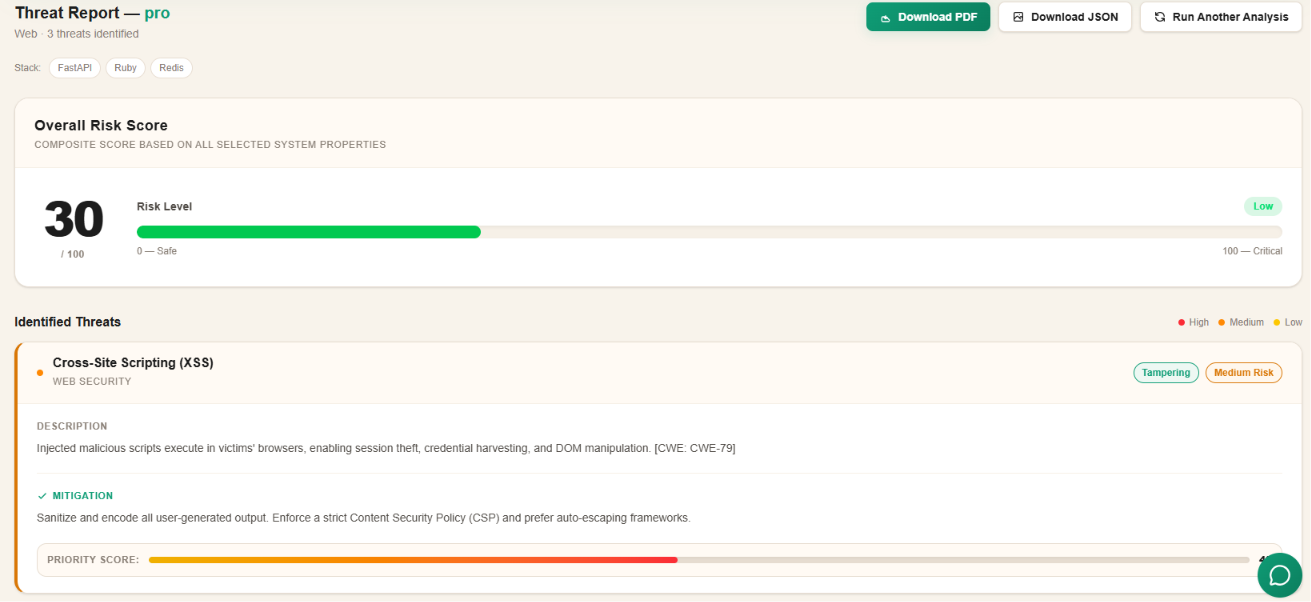
\includegraphics[width=\textwidth]{media/Threat Modeling Analysis.png}
\caption{Threat Modeling Analysis}
\label{fig:ch6_threat_modeling_analysis}
\end{figure}

\subsection{Reviewing Threat Modeling Results}

Results present categorised threats with descriptions, mitigations, and risk ratings. AI-assisted explanations supplement rule-based analysis.

Each threat entry includes category, severity, description, affected component, and recommended mitigation controls.

\subsection{Exporting Threat Model Reports}

Download threat model reports as client-side generated PDF from the results page.

PDF generation executes entirely in the browser without server-side rendering, producing a formatted document from the current analysis state.

\subsection{Saved Threat Models and History}

Saved models are accessible from history and Reports History for retrospective review and comparison.

Saved models retain the application profile and generated threat set for retrospective comparison across design iterations.

\section{AI Malware Analysis}

AI Malware Analysis performs static PE classification and AI-generated SOC reporting at /dashboard/ai-malware-analysis for .exe, .dll, and .sys files (max 512 MB). Files are analysed without execution; classification is based on extracted static PE features.

\subsection{AI Malware Analysis Module Overview}

The module extracts static PE features, classifies malware probability, and optionally generates Gemini-powered SOC reports with PDF export.

Analysis is static only; uploaded files are not executed in a sandbox environment. The module employs a two-stage PE malware classifier for probability scoring.

\subsection{Uploading and Submitting a File}

Upload PE executables via drag-and-drop or file selector. Alternatively, submit pre-extracted JSON feature payloads for classification.

Drag-and-drop and file selector interfaces accept .exe, .dll, and .sys files. JSON mode accepts the 47 static PE feature fields for direct classification.

\begin{figure}[H]
\centering
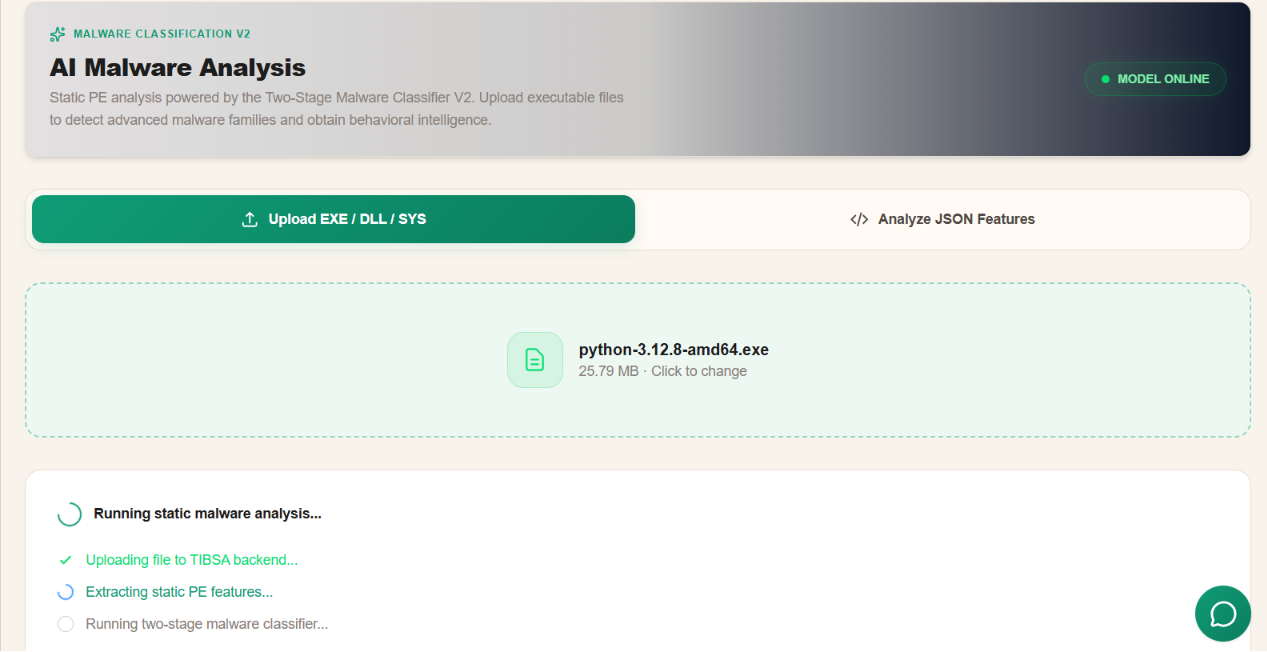
\includegraphics[width=\textwidth]{media/AI Malware Analysis Upload.png}
\caption{AI Malware Analysis Upload}
\label{fig:ch6_ai_malware_analysis_upload}
\end{figure}

\subsection{Malware Analysis Pipeline Execution}

Static feature extraction and classification execute upon upload. Progress stages are displayed during processing.

Feature extraction parses PE headers, sections, imports, and entropy metrics before classification model inference.

\subsection{Reviewing Analysis Results}

Results display malware probability, verdict, feature summary, and classification metadata. Invalid PE files are rejected with an error message.

The results panel presents malware probability percentage, binary verdict, and extracted metadata including compile timestamp and section characteristics.

\subsection{AI-Powered Malware Explanation}

Generate an AI SOC report from static results. The report includes executive summary, technical findings, and recommendations.

SOC report generation invokes the Gemini integration, producing structured sections including executive summary, indicators, and recommended response actions.

\subsection{Exporting Malware Analysis Reports}

Download AI-generated PDF reports when generation succeeds. Session state persists in browser sessionStorage.

PDF download is available when AI report generation succeeds. Failed generation displays a notification while static results remain accessible.

\subsection{Session History and Previous Analyses}

Backend history and localStorage session records enable retrieval of prior analyses within the module workspace.

Backend history retrieves prior scans via the module API; local session records supplement persistence within the current browser session.

\section{Reports History}

Reports History at /dashboard/reports aggregates completed outputs from Security Investigations, Penetration Testing, Security Scans, and Threat Modeling.

\subsection{Reports History Overview}

The module provides tabbed navigation with record counts per category. It does not initiate new analyses; it surfaces persisted outputs from originating modules.

On page load, four concurrent API requests populate tab counts for each report category, providing immediate visibility into available historical records.

\begin{figure}[H]
\centering
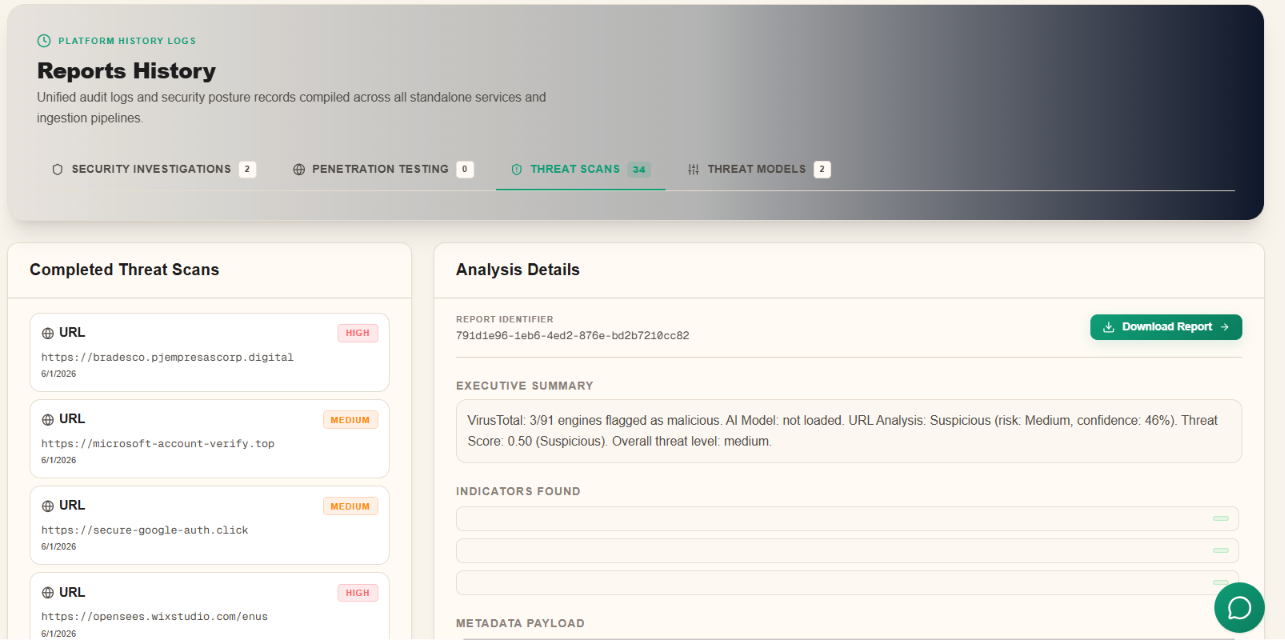
\includegraphics[width=\textwidth]{media/Reports History Interface.png}
\caption{Reports History Interface}
\label{fig:ch6_reports_history_interface}
\end{figure}

\subsection{Available Report Categories}

Table~\ref{tab:ch6_reports_history_categories} summarises report categories, source modules, and primary access paths.

\begin{table}[H]
\centering
\caption{Reports History Categories}
\label{tab:ch6_reports_history_categories}
\begin{tabular}{lll}
\toprule
\textbf{Category} & \textbf{Source Module} & \textbf{Access Path} \\
\midrule
Security Investigations & Investigations pipeline & /dashboard/investigations/\{id\} \\
Penetration Testing & Website scanner & /dashboard/website-scanner \\
Threat Scans & Security Scans & /dashboard/scans \\
Threat Models & Threat Modeling & /dashboard/threat-modeling \\
\bottomrule
\end{tabular}
\end{table}

\subsection{Accessing Historical Results}

Select a tab and row to navigate to the authoritative module workspace for detailed review. Threat scan entries open the scan detail modal; investigation entries route to the live investigation page.

Empty tabs indicate no completed analyses exist for that category. Users should complete at least one analysis in the source module to populate history.

\section{User Profile \& Notifications}

\subsection{User Profile}

The Profile page at /dashboard/profile displays read-only account information including full name, email, role, and account status retrieved from GET /api/v1/users/me.

Profile fields are read-only in the current implementation; account modifications require administrator intervention through SOC Nexus User Management.

\subsection{Notification System}

Platform notifications appear in the header bell dropdown, refreshed every fifteen seconds. Users mark notifications read individually or in bulk. Notification types include threat, scan, and system events.

Unread notifications display a count badge on the bell icon. The dropdown supports mark-all-read for bulk notification management.

\section{Administration (SOC Nexus)}

The SOC Nexus admin console at /admin is restricted to users with the admin role.

\subsection{Administrative Dashboard}

The overview dashboard presents user counts, active sessions, threat indicators, and platform activity summaries with optional live-refresh toggles.

Live dashboard refresh can be toggled via localStorage preference. Key metrics include total users, active sessions, and recent platform activity.

\begin{figure}[H]
\centering
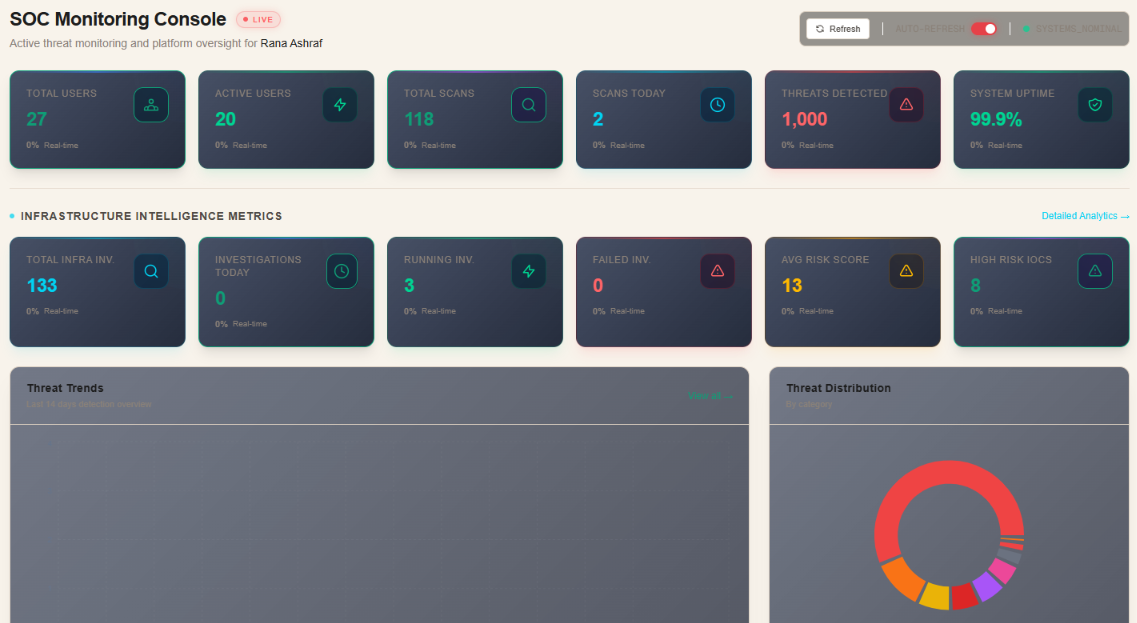
\includegraphics[width=\textwidth]{media/SOC Nexus Admin Dashboard.png}
\caption{SOC Nexus Admin Dashboard}
\label{fig:ch6_soc_nexus_admin_dashboard}
\end{figure}

\subsection{User and Threat Management}

User Management supports viewing, searching, role assignment, and account activation/deactivation. Threat Feed Management displays configured intelligence feeds with status, indicator counts, and reliability scores.

Administrators may deactivate accounts, triggering immediate access revocation and redirection to the suspended-account page for affected users.

\subsection{Monitoring and Analytics}

Platform Analytics and Infra Intelligence Analytics provide usage trends and investigation statistics. System Health Monitoring displays service status. The Audit Log records authentication events, scan creation, and admin actions.

Audit log entries record action type, severity, timestamp, IP address, and user agent for security-relevant events across the platform.

\subsection{System Configuration}

Platform Settings manage toggles (audit logging, API access) and numeric inputs (rate limits, session timeout). Settings persist via the backend admin settings API.

Configurable parameters include rate limits, session timeout, and maximum upload size. Email alerts toggle is displayed but disabled by default.

\section{AI Features}

AI capabilities are integrated across multiple modules rather than operating as a standalone service.

Security Investigations generate AI executive summaries upon pipeline completion. Infra Intelligence produces AI infrastructure reports. AI Malware Analysis generates Gemini-powered SOC reports from static classification results. Threat Modeling supplements rule-based threats with AI explanations. The floating AI Security Assistant provides conversational guidance across dashboard routes.

AI-generated outputs should be validated by analysts; they supplement but do not replace deterministic scan and classification results. AI report availability depends on successful integration with configured language model services.

The AI Security Assistant operates independently of module-specific AI reporting, providing general security guidance rather than analysis of submitted indicators.

\section{Report Export Reference}

Table~\ref{tab:ch6_export_format_reference} summarises export formats available across implemented modules. Export controls appear on module detail pages upon completion of the relevant analytical pipeline. Users should ensure analysis status is completed before attempting export operations.

\begin{table}[H]
\centering
\caption{Export Format Reference}
\label{tab:ch6_export_format_reference}
\begin{tabular}{lll}
\toprule
\textbf{Module} & \textbf{Formats} & \textbf{Purpose} \\
\midrule
Security Investigations & JSON, PDF & Structured data and executive reporting \\
Infra Intelligence & PDF, JSON & Infrastructure investigation archival \\
Threat Modeling & PDF & STRIDE threat model documentation \\
AI Malware Analysis & PDF & AI SOC report download \\
Penetration Testing & JSON & Scan findings interchange \\
Security Scans & --- & In-module result review \\
Audit Log (Admin) & CSV & Compliance export \\
\bottomrule
\end{tabular}
\end{table}

\section{Investigation Types and Target Matrix}
\label{sec:ch6_investigation_matrix}

Table~\ref{tab:ch6_investigation_types_target_matrix} maps modules to supported investigation target types for module selection.

\subsection{Investigation Types Overview}

TIBSA provides specialised modules for vulnerability assessment, threat intelligence, malware analysis, and architectural threat modelling. Module selection should align with the indicator type and investigation objective.

Vulnerability assessment modules (Security Investigations, Penetration Testing) evaluate web application security. Threat intelligence modules enrich infrastructure indicators. Malware analysis classifies executables. Threat Modeling assesses design.

\subsection{Supported Target Types}

Supported targets include URL, domain, IP address, file hash (MD5/SHA-1/SHA-256), email address, and file upload (PE executables for malware analysis; general files for Security Scans).

URL targets require explicit scheme prefixes for scan modules. Hash targets accept hexadecimal strings of standard lengths (32, 40, or 64 characters).

\subsection{Investigation Types and Target Matrix}

\begin{table}[H]
\centering
\caption{Investigation Types and Target Matrix}
\label{tab:ch6_investigation_types_target_matrix}
\begin{tabular}{lcccccc}
\toprule
\textbf{Module} & \textbf{URL} & \textbf{Domain} & \textbf{IP} & \textbf{Hash} & \textbf{Email} & \textbf{File Upload} \\
\midrule
Security Investigations & $\checkmark$ & --- & --- & --- & --- & --- \\
Infra Intelligence & $\checkmark$ & $\checkmark$ & $\checkmark$ & $\checkmark$ & $\checkmark$ & --- \\
Security Scans & $\checkmark$ & --- & --- & $\checkmark$ & --- & $\checkmark$ \\
Penetration Testing & $\checkmark$ & --- & --- & --- & --- & --- \\
Threat Intelligence Lookup & $\checkmark$ & $\checkmark$ & $\checkmark$ & $\checkmark$ & $\checkmark$ & --- \\
AI Malware Analysis & --- & --- & --- & --- & --- & $\checkmark$ \\
\bottomrule
\end{tabular}
\end{table}

\subsection{Module Selection Guidelines}

Route suspicious websites to Security Investigations or Penetration Testing; infrastructure indicators to Infra Intelligence or Threat Intelligence Lookup; executables to AI Malware Analysis; design reviews to Threat Modeling.

When comprehensive assessment is required, Security Investigations orchestrates multiple stages; standalone modules provide focused analysis of single aspects.

\subsection{Cross-Module Investigation Strategy}

Complex investigations may chain Threat Intelligence Lookup, Infra Intelligence, Security Investigations, and Malware Analysis sequentially, with Reports History providing unified visibility.

Integrated analysis supports SOC triage workflows: rapid lookup, deep enrichment, vulnerability assessment, and malware classification within a unified environment.

\section{Chapter Summary}

The TIBSA platform provides an integrated analyst workflow commencing with authentication and navigation through the TIBSA Shield interface. Analysts launch investigations via the main dashboard into Security Investigations (URL pipelines), Infra Intelligence (IOC enrichment), or AI Malware Analysis (static PE classification). Standalone services---Security Scans, Penetration Testing, Threat Intelligence Lookup, and Threat Modeling---address specific assessment requirements. Reports History consolidates completed outputs; administrators manage the platform through SOC Nexus.

Module selection should follow the investigation target type and analytical objective as defined in Section~\ref{sec:ch6_investigation_matrix}. AI-assisted reporting supplements deterministic findings across investigations, infrastructure analysis, malware classification, and threat modelling workflows.

Operational success depends on selecting the appropriate module for each indicator type, allowing analytical pipelines to complete before export, and consulting Reports History for unified visibility across prior assessments. Administrators maintain platform integrity through user management, audit review, and system configuration within SOC Nexus.

